\documentclass[]{report}
\usepackage{kotex}
\usepackage{verbatim} 
\usepackage{graphicx} 

\usepackage{listings}
\usepackage{color}

\definecolor{dkgreen}{rgb}{0,0.6,0}
\definecolor{gray}{rgb}{0.5,0.5,0.5}
\definecolor{mauve}{rgb}{0.58,0,0.82}

\lstset{frame=tb,
	language=Python,
	aboveskip=3mm,
	belowskip=3mm,
	showstringspaces=false,
	columns=flexible,
	basicstyle={\small\ttfamily},
	numbers=none,
	numberstyle=\tiny\color{gray},
	keywordstyle=\color{blue},
	commentstyle=\color{dkgreen},
	stringstyle=\color{mauve},
	breaklines=true,
	breakatwhitespace=true,
	tabsize=3
}


% Title Page
\title{HW03 - REPORT}
\author{정보컴퓨터공학부 201624536 이국현}


\begin{document}
	\maketitle
	
	
\chapter{서론}
\begin{itemize}
	\item Noise Reduction
	\item Image Derivatives
	\item Non-Maximum Suppression
	\item Threshold
	\item Edge Tracking
\end{itemize} 

\section{Image Derivatives}

\subsection{Edge의 특성}

\begin{figure}[ht!]
	\centering
	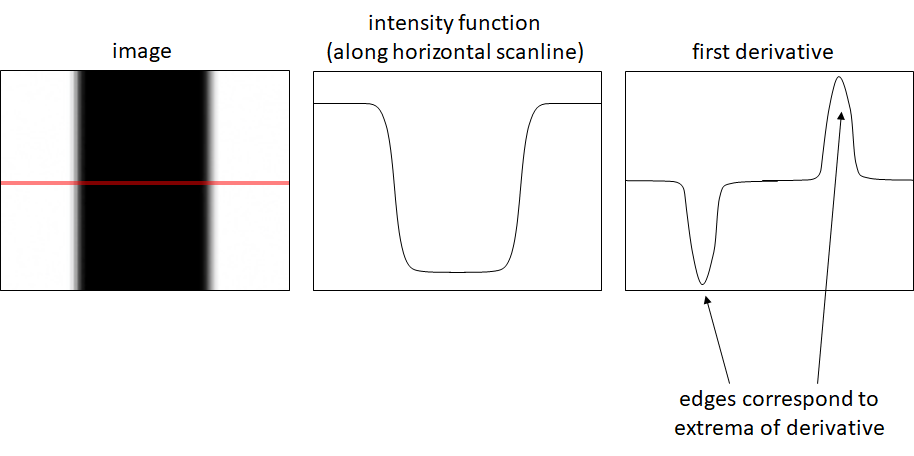
\includegraphics[width=0.9\textwidth]{image/1-1.png}
	\caption{Image Derivatives}
	\label{1-1}
\end{figure}

Edge에서는 Pixel의 변화량이 클 것이다. 따라서 우리는 Image Intensity가 급격하게 변하는 부분을 찾아 Edge를 추출할 수 있다. \\

\subsection{Image Derivatives}
Discreate Pixel을 X, Y에 대해서 각각 편미분을 구한다. \\
\[ I_x = \frac{\partial f}{\partial x} \approx F[x+1, y] - F[x, y] \] \\
\[ I_y = \frac{\partial f}{\partial x} \approx F[x, y+1] - F[x, y] \] \\

X, Y에 대해서 변화량이 큰 Pixel은 Edge가 된다. \\


\subsection{with Convolution}
\begin{figure}[ht!]
	\centering
	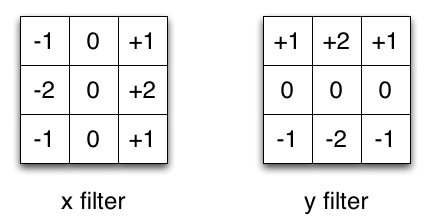
\includegraphics[width=0.9\textwidth]{image/1-2.png}
	\caption{Derivative Kernel}
	\label{1-2}
\end{figure}


\section{Noise Reduction}
\subsection{Noise}

\begin{figure}[ht!]
	\centering
	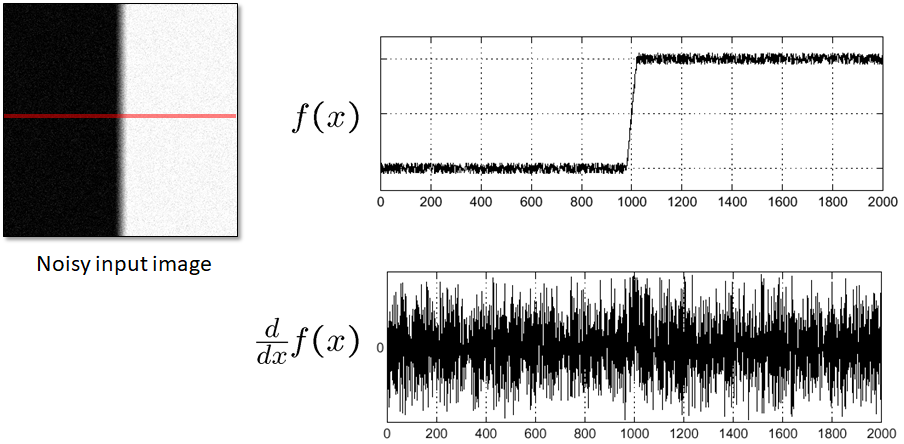
\includegraphics[width=0.9\textwidth]{image/1-3.png}
	\caption{Noise}
	\label{1-3}
\end{figure}

실제 이미지에서는 Edge가 아주 매끄럽게 구분되는 것이 아니기 때문에 Noise가 생기고, 이 때문에 Edge를 추출하는 것이 어려워진다. \\

\subsection{Solution : smooth}

\begin{figure}[ht!]
	\centering
	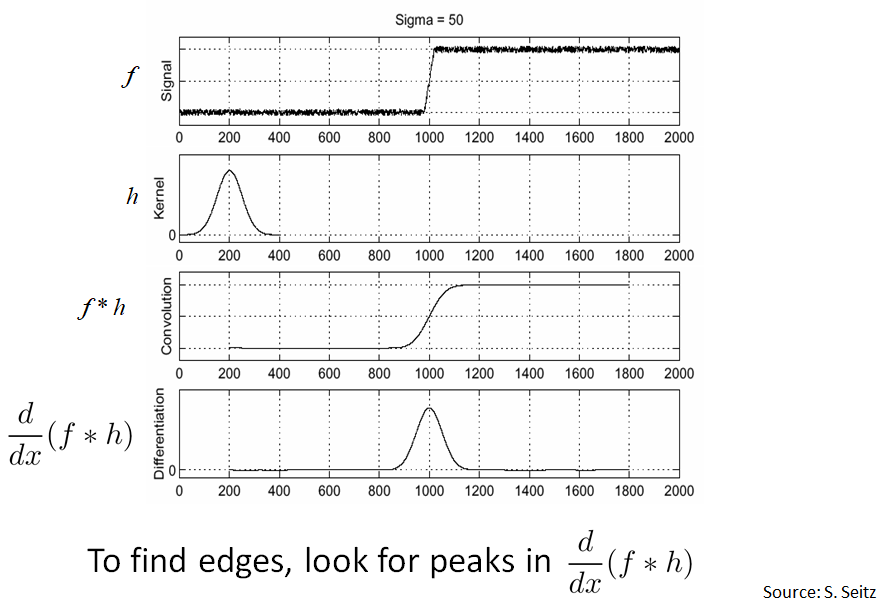
\includegraphics[width=0.9\textwidth]{image/1-4.png}
	\caption{smooth}
	\label{1-4}
\end{figure}

우리는 Edge에서 Noise를 줄이기 위해 Detail 부분을 없애고 Blur 효과를 주는 Gaussian Filter를 Convolution할 수 있다. Convolution은 Associative한 특성이 있기 때문에 앞에서 살펴 본 Derivate Kernel과 순서를 바꾸어 적용할 수 있다. \\



\section{Non-Maximum Suppression}

Image Intensity 값에 따라 Pixel을 Edge로 표시하였지만, Image가 Blur 처리되어 있기 때문에, Edge가 너무 굵을 수 있다. 각 Pixel의 Gradient Direction에서 maximum이면 값을 살리고 아니면 없애 얇고 선명한 Edge를 구할 수 있다. \\

\section{Threshold}

\begin{itemize}
	\item Strong Edge $( T_{high} < R )$
	\item Weak Edge $(T_{low} < R < T_{high})$
	\item No Edge $(R < T_{low})$
\end{itemize} 

Non-maximum supression을 수행한 이미지에도 여전히 Noise가 남아 있다. 그래서 2가지 Threshold $T_{high}, T_{low}$를 두고 Pixel을 위와 같이 3가지로 분류한다. \\

\section{Edge Tracking}

Strong Edge와 연결된 Weak Edge는 모두 Strong Edge로 바꿔주고, 나머지 모든 Weak Edge는 제거한다. \\



\chapter{본론}

\section*{Prob 1: Noise Reduction}

\begin{lstlisting}
def problem1():
	img = Image.open(IMAGE_PATH)
	imgGrey = img.convert('L')
	arrayGrey = np.asarray(imgGrey)
	arrayGreyBlur = gaussconvolve2d(arrayGrey, SIGMA)
	arrayToImg(arrayGreyBlur, 'problem1.png')
	return arrayGreyBlur
\end{lstlisting}

Edge를 추출할 때 Noise를 제거하기 위해 Image에 Gaussian Convolution을 통해 Blur 처리를 해주었다. \\

\begin{figure}[ht!]
	\centering
	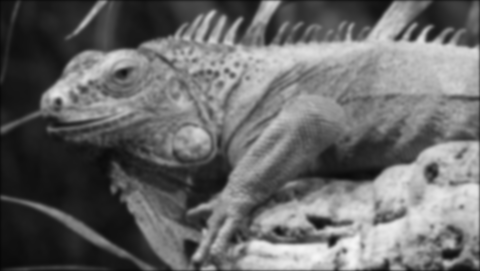
\includegraphics[width=0.9\textwidth]{image/problem1.png}
	\caption{Blur Image}
	\label{problem1}
\end{figure}

\section*{Prob 2: Intensity Gradient}

\begin{lstlisting}
def sobel_filters(img):
	# Derivate Kernel을 Convolution하여 Ix, Iy 구함
	IxKernel = np.array([[-1, 0, 1], [-2, 0, 2], [-1, 0, 1]])
	IyKernel = np.array([[1, 2, 1], [0, 0, 0], [-1, -2, -1]])
	Ix = convolve2d(img, IxKernel)
	Iy = convolve2d(img, IyKernel)
	
	G = np.hypot(Ix, Iy) # sqrt(Ix^2 + Iy^2)
	theta = np.arctan2(Iy, Ix) # tan^(-1)(Iy / Ix)
	
	# mapping (0 to 255)
	maxVal = G.max()
	minVal = G.min()
	G = (G * 255) / (maxVal - minVal)
	return (G, theta)
\end{lstlisting}

Pixel 값을 Derivate Kernel을 Convolution하여 Ix, Iy를 구하고, Gradient Intensity를 G, Gradient Direction을 theta에 저장하였다. 이때 Gradient Intensity를 Edge로 시각화하기 위해 값을 0 ~ 255 범위로 변환하였다. \\

\begin{figure}[ht!]
	\centering
	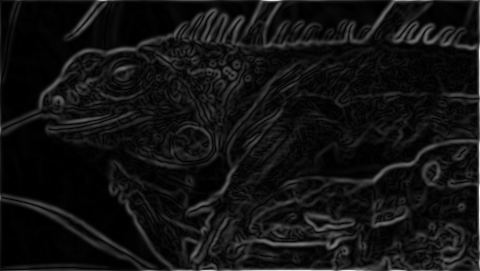
\includegraphics[width=0.9\textwidth]{image/problem2.png}
	\caption{Visualize Gradient Intensity}
	\label{problem2}
\end{figure}

\section*{Prob 3: Non-Maximum Suppression}

\begin{lstlisting}
def getDirection(degree):
	# 가장 가까운 방향을 찾아냄
	directionArray = np.array([0, 45, 90, 135, 180])
	index = (np.abs(directionArray - degree)).argmin()
	return directionArray[index % 4]

def non_max_suppression(G, theta):
	# reduce range : 2 * pi => pi
	theta = (theta + np.pi) % np.pi
	# radian to degree
	degrees = theta * 180 / np.pi

	thinEdge = np.zeros(G.shape)
	ySize, xSize = G.shape
	for y in range(1, ySize - 1): # 이미지 끝 부분은 제외
		for x in range(1, xSize - 1):
			areaG = G[y - 1 : y + 2, x - 1 : x + 2]
			# degree에 따라 확인할 target 변경
			degree = getDirection(degrees[y][x])
			target = np.array([0, 0, 0])
			if(degree == 0):     target = areaG[1, :]
			elif(degree == 45):  target = np.diag(np.fliplr(areaG))
			elif(degree == 90):  target = areaG[:, 1]
			elif(degree == 135): target = np.diag(areaG)
			else: assert True, "direction is not valid"
	
			# pixel이 지정 방향에서 max gradient를 가지는지 확인
			if(target.argmax() == 1):
				thinEdge[y][x] = G[y][x]
	return thinEdge
\end{lstlisting}

Prob2에서 구한 G를 theta 방향에서 Maximum Gradient를 가질 때만 Pixel을 남기고 나머지는 제거했다. 여기서 방향은 거꾸로 해도 같기 때문에 각도 범위를 0 ~ pi로 변환하였다. 그리고 상하, 좌우, 대각선, 반대 대각선 중 가장 가까운 방향으로 확인하도록 구현하였다. \\

\begin{figure}[ht!]
	\centering
	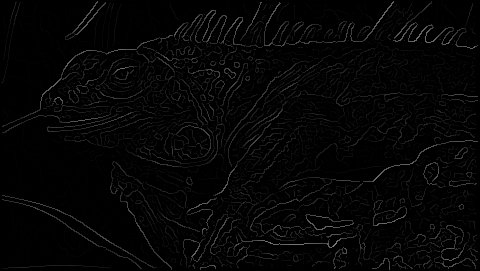
\includegraphics[width=0.9\textwidth]{image/problem3.png}
	\caption{Non-Maximum Suppression}
	\label{problem3}
\end{figure}

\section*{Prob 4: Threshold}

\begin{lstlisting}
def double_thresholding(img):
	diff = img.max() - img.min()
	highT = img.min() + diff * 0.15
	lowT = img.min() + diff * 0.03
	thresholded = np.where(img > highT, STRONG, img)
	thresholded = np.where((img > lowT) & (img <= highT), WEAK, thresholded)
	thresholded = np.where(img <= lowT, 0, thresholded)
	return thresholded
\end{lstlisting}

Non-Maximum Suppression을 적용한 이미지에 threshold를 통해 Strong Edge(255), Weak Edge(80), No-Edge(0)으로 구분하였다. \\

\begin{figure}[ht!]
	\centering
	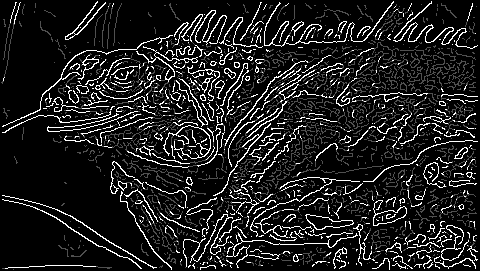
\includegraphics[width=0.9\textwidth]{image/problem4.png}
	\caption{Threshold}
	\label{problem4}
\end{figure}


\section*{Prob 5: Edge Tracking}

\begin{lstlisting}
def DFS(img, centerY, centerX):
	ySize, xSize = img.shape
	# 이미지 끝 부분은 제외
	if(centerY <= 0 or centerX <= 0 or centerY >= ySize - 1 or centerX >= xSize - 1):
		return
	# 연결된 모든 weak edge를 strong edge로 변환
	for y in range(centerY - 1, centerY + 2):
		for x in range(centerX - 1, centerX + 2):
			if(img[y][x] == WEAK):
				img[y][x] = STRONG
				DFS(img, y, x)

def hysteresis(img):
	# 모든 strong edge를 순회하여 DFS
	strongY, strongX = np.where(img == STRONG)
	for i in range(len(strongY)):
		DFS(img, strongY[i], strongX[i])
	# 나머지 weak edge는 제거
	img = np.where(img == WEAK, 0, img)
	return img
\end{lstlisting}

Strong Edge를 구성하는 Pixel에서 DFS를 수행해 연결된 모든 Weak Edge를 Strong Edge로 변환해 주었다. 그리고 Strong Edge가 되지 못한 나머지 Weak Edge는 제거하였다. \\

\begin{figure}[ht!]
	\centering
	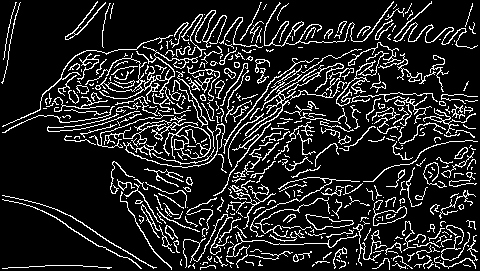
\includegraphics[width=0.9\textwidth]{image/problem5.png}
	\caption{Edge Tracking}
	\label{problem5}
\end{figure}

\chapter{결론}

지금까지 5단계에 걸쳐 Canny Edge Detector를 구현해 보았다. 서론과 달리 코드에서는 먼저 Noise 제거를 위한 Gaussian Filter를 Convolution 해주었는데, 이는 Convolution 연산이 Associative한 속성을 가지고 있기 때문이다. 따라서 이를 잘 활용하면 이미지 처리에 연산량을 크게 줄일 수 있다. \\

Canny Edge Detector를 통해 Edge를 추출할 수 있었지만, 이미지의 상태에 따라서 확실한 Edge를 추출하기 어려울 수 있다. 따라서 Noise 제거에 사용하는 Sigma, Edge Filtering을 위한 Threshold 값을 잘 조절하여 사용하여야 한다. \\ 


\end{document}          
